 \makeatletter
\renewcommand{\cleardoublepage}{\clearpage} % Evita páginas en blanco extra
\makeatother

%\frontmatter % Use roman page numbering style (i, ii, iii, iv...) for the pre-content pages

%\pagestyle{plain} % Default to the plain heading style until the thesis style is called for the body content

% --- UFPE: contar desde a folha de rosto, sem numerar o pré-texto ---
%\pagenumbering{arabic}  % contador en arábigos desde el comienzo
%\pagestyle{empty}       % no mostrar número en las páginas por ahora

%----------------------------------------------------------------------------------------
%	TITLE PAGE
%----------------------------------------------------------------------------------------


\begin{titlepage}
  \begin{center}
  
    % LOGO ARRIBA
    % Ajusta la ruta y el tamaño de tu logo (o quítalo si no quieres poner imagen)
			$if(thesis.logo)$
			$if(thesis.logo-height)$
			\includegraphics[height=$thesis.logo-height$]{$thesis.logo$} % University/department logo
			$else$
			\includegraphics{$thesis.logo$}
			$endif$
			$endif$\\[0.3cm]
    %
\includegraphics[width=2cm]{images/ufpe-logo.png}\\[0.3cm]
    
    % NOMBRES DE LA UNIVERSIDAD/PROGRAMA EN MAYÚSCULAS
    {\normalsize\MakeUppercase{UNIVERSIDADE FEDERAL DE PERNAMBUCO}}\\
    {\normalsize\MakeUppercase{CENTRO DE CIÊNCIAS EXATAS E DA NATUREZA}}\\
    {\normalsize\MakeUppercase{PROGRAMA DE PÓS-GRADUAÇÃO EM ESTATÍSTICA}}\\ [4cm]
    %{\large\MakeUppercase{DOUTORADO EM ESTATÍSTICA}}\\[4cm]
		
    % NOMBRE DE LA TESISTA
    {\normalsize ROSA JANETH ALPALA}\\[4cm]
    
    % TÍTULO 
    {\normalsize \textbf{ENTROPY-BASED TEST STATISTICS FOR HETEROGENEITY DETECTION IN SAR DATA}}\\[6.19cm]
    %\textbf{AND CAUSE-SPECIFIC MORTALITY IN ENGLAND}}\\[5cm]
    % Entropy-Based Test Statistics for Heterogeneity Detection in SAR Data

		
		%{\Large Doctoral Thesis}\\[2cm] % Thesis type
%
    % CIUDAD Y AÑO
    %\vfill
   {\normalsize Recife}\\
   {\normalsize 2025}
    
  \end{center}
\end{titlepage} % <— FIN de la portada
\cleardoublepage

% --- Aquí COMIENZA el conteo (folha de rosto = 1), pero sin imprimir número ---
\pagenumbering{arabic}   % resetea a 1 en esta página
\pagestyle{empty}        % no mostrar números en el pretexto

\begin{titlepage}
  \thispagestyle{empty}
    \begin{center}
    {\normalsize ROSA JANETH ALPALA}\\[5cm]
    {\normalsize \textbf{ENTROPY-BASED TEST STATISTICS FOR HETEROGENEITY DETECTION IN SAR DATA}}\\[3cm]
  \end{center}

  % Quita el \hfill y en lugar de eso usamos \begin{center}...
  %\begin{center}
  \noindent
  \hspace*{0.44\textwidth}
  \begin{minipage}{0.52\textwidth}
  \onehalfspacing
  Tese apresentada ao Programa de Pós-Graduação em Estatística do Centro de Ciências
  Exatas e da Natureza da Universidade Federal
  de Pernambuco, como requisito parcial à
  obtenção do título de Doutora em Estatística.
    % Thesis submitted to the Graduate Program in Statistics at 
    % the Universidade Federal de Pernambuco, as a partial requirement 
    % for the degree of Doctor of Philosophy  in Statistics.
   % \end{minipage}
    
      %\hspace*{0.34\textwidth}% \hspace*{0.34\textwidth}
 % \begin{minipage}{0.65\textwidth}%\begin{minipage}{0.65\textwidth}
  \vspace{2em}
    %\textbf{Concentration area}: Applied Statistics
    \textbf{Área de Concentração}: Estatística Aplicada
    
    \vspace{2em} 
    \textbf{Orientador}: Dr. Alejandro César Frery Orgambide \\
    \textbf{Co-Orientador}: Dr. Abraão David Costa do Nascimento
  \end{minipage}
  %\end{center}
  
  \vfill
  \begin{center}
    Recife\\
    2025
  \end{center}
\end{titlepage}
\setcounter{page}{2}
% --- Folha em branco para a ficha catalográfica (contada, sem número) ---
\clearpage
\thispagestyle{empty}
\null
\newpage


 % la Capa NO se cuenta; la próxima hoja será la 1

% --- SUBPORTADA O FOLHA DE ROSTO ---

% \begin{titlepage}
%   \thispagestyle{empty} % Quita numeración en esta página
%   
%   \begin{center}
%     % --- NOMBRE DEL ESTUDIANTE --- 
%     {\large ROSA JANETH ALPALA}\\[3cm]
%     
%     % --- TÍTULO EN MAYÚSCULAS O NEGRITA --- 
%     {\Large \textbf{TEST STATISTICS BASED ON ENTROPY FOR HETEROGENEITY DETECTION IN SAR DATA }}\\[3cm]
%     %\textbf{}}\\[3cm]
%   \end{center}
% %Test Statistics Based on Entropy and the Coefficient of Variation for Heterogeneity Detection in SAR Data
%   \hfill
%   \begin{minipage}{0.6\textwidth}
%     % -- TEXTO DESCRIPTIVO --
%     Thesis submitted to the Graduate Program in Statistics of the Universidade Federal de Pernambuco, as a partial requirement for the degree of Doctor in Statistics.
%     
%     \vspace{1em}
%     \textbf{Concentration area}: Applied Statistics
%     
%     \vspace{2em} 
% 		\textbf{Advisor}: Prof. Alejandro C. Frery \\
% 		\textbf{Co-advisor}: Prof. Abraão David Costa do Nascimento
%    
%   \end{minipage}
%   
%   \vfill
%   \begin{center}
%     Recife\\
%     2025
%   \end{center}
% 
% \end{titlepage}

% --- ACTA en PDF (contada, sin número visible) ---

\cleardoublepage
% (opcional) marcador de PDF sin añadir al ToC:
%\phantomsection
%\pdfbookmark[0]{ACTA}{acta}

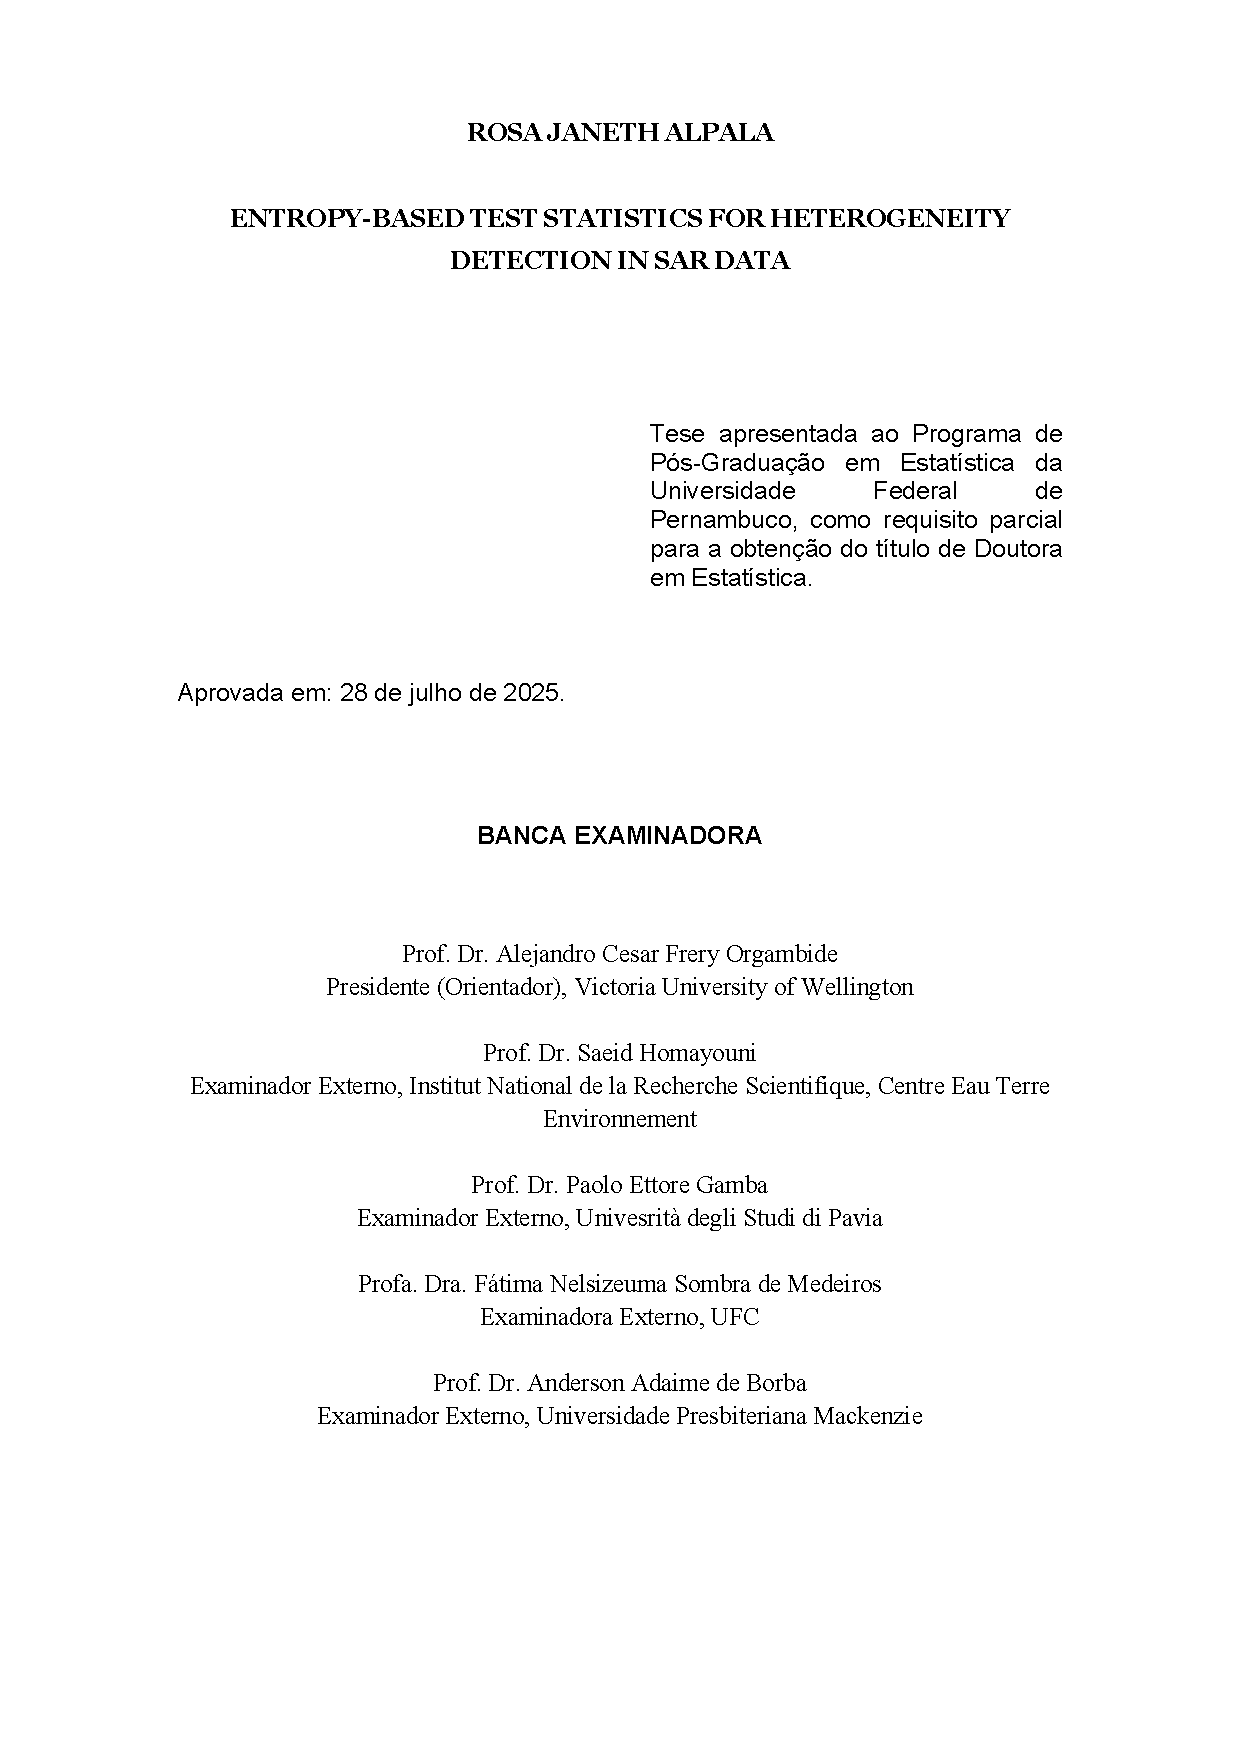
\includepdf[
  pages=-,                    % todas las páginas del PDF
  pagecommand={\thispagestyle{empty}}, % oculta el número en cada página incluida
  fitpaper=true               % ajusta al tamaño del papel del documento
]{Frontmatter/Folha2.pdf}

\cleardoublepage


%----------------------------------------------------------------------------------------
%	Actas
%----------------------------------------------------------------------------------------
%\cleardoublepage % Asegura que la portada termine en una página aparte
%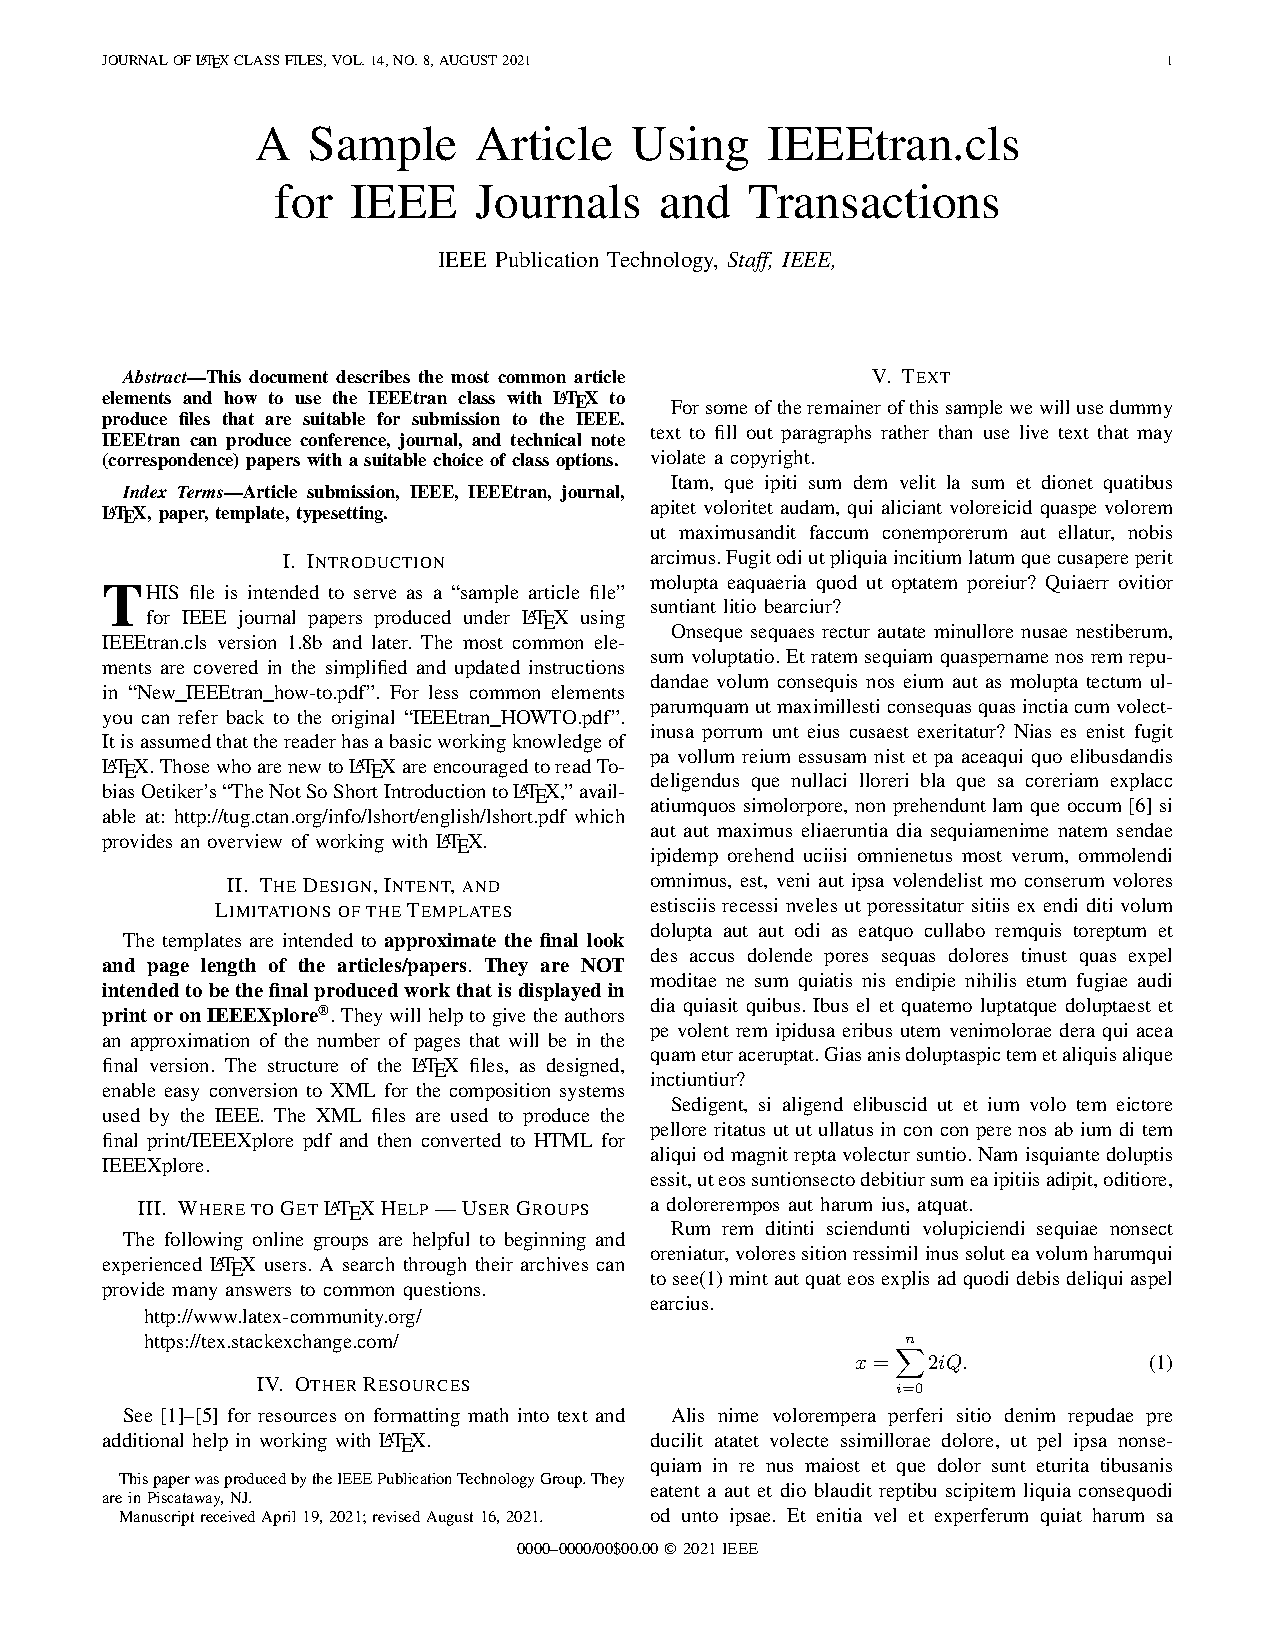
\includepdf[pages=-]{Frontmatter/acta.pdf}
%\cleardoublepage
% Pretexto: no mostrar número

\pagestyle{empty}
\setchapterpagestyle{empty} % las "chapter pages" del pretexto también sin número


$if(thesis.dedication)$
%----------------------------------------------------------------------------------------
%	DEDICATION
%----------------------------------------------------------------------------------------

%\dedicatory{\input{"$thesis.dedication$"}} 
\dedicatory{\vfill}{\input{"$thesis.dedication$"}}

$endif$

$if(thesis.acknowledgements)$
%----------------------------------------------------------------------------------------
%	ACKNOWLEDGEMENTS
%----------------------------------------------------------------------------------------

%\begin{acknowledgements}
%%\addchaptertocentry{\acknowledgementname} % Add the acknowledgements to the table of contents
%$if(thesis.acknowledgements.text)$
%$thesis.acknowledgements.text$
%$else$
%\input{"$thesis.acknowledgements$"}
%$endif$
%\end{acknowledgements}
%
%$endif$
 

$if(thesis.acknowledgements)$
\begingroup
\renewcommand{\abovechapterskip}{\vspace*{15pt}}  % En lugar de 20pt
  \renewcommand{\chapterbelowskip}{\vspace*{20pt}}  % En lugar de 40pt
  % Aquí redefinimos las macros solo para este entorno
  \renewcommand{\chapteralign}{\centering}      % Centra el título
  \renewcommand{\chapterfont}{\bfseries\Large}  % Negrita y tamaño grande (ajusta a gusto)

  \begin{acknowledgements}
  \thispagestyle{empty} 
  %\addchaptertocentry{\acknowledgementname} % Add the acknowledgements to the table of contents
  
  $if(thesis.acknowledgements.text)$
  $thesis.acknowledgements.text$
  $else$
  \input{"$thesis.acknowledgements$"}
  $endif$

  \end{acknowledgements}
\endgroup
$endif$

%%----------------------------------------------------------------------------------------
%%	DECLARATION PAGE
%%----------------------------------------------------------------------------------------
%$if(thesis.declaration)$
%\begin{declaration}
%\addchaptertocentry{\authorshipname} % Add the declaration to the table of contents
%$if(thesis.declaration.text)$
%$thesis.declaration.text$
%$else$
%\input{"$thesis.declaration$"}
%$endif$
%
%\end{declaration}
%
%\cleardoublepage
%$endif$
%
%$if(thesis.quotation)$
%%----------------------------------------------------------------------------------------
%%	QUOTATION PAGE
%%----------------------------------------------------------------------------------------
%
%\vspace*{0.2\textheight}
%
%$if(thesis.quotation.text)$
%\noindent``{\itshape $thesis.quotation.text$}''\bigbreak
%
%\hfill $thesis.quotation.attribution$
%$else$
%\input{``$thesis.quotation$''}
%$endif$
%
%$endif$

%$if(abstract)$
%%----------------------------------------------------------------------------------------
%%	ABSTRACT PAGE
%%----------------------------------------------------------------------------------------
%
%\begin{abstract}
%\addchaptertocentry{\abstractname} % Add the abstract to the table of contents
%$abstract$
%\end{abstract}
%
%$endif$


$if(thesis.abstract)$
\begingroup
\renewcommand{\abovechapterskip}{\vspace*{10pt}}  % En lugar de 20pt
  \renewcommand{\chapterbelowskip}{\vspace*{10pt}}  % En lugar de 40pt
  % Aquí redefinimos las macros solo para este entorno
  \renewcommand{\chapteralign}{\centering}      % Centra el título
  \renewcommand{\chapterfont}{\bfseries\Large}  % Negrita y tamaño grande (ajusta a gusto)
\begin{abstract}
 \thispagestyle{empty}  
\input{"$thesis.abstract$"} 
\end{abstract}
\newpage % Solo inserta nueva página si es necesario
\endgroup
$endif$

$if(thesis.resumo)$
\begingroup
 \renewcommand{\abovechapterskip}{\vspace*{10pt}}  % En lugar de 20pt
  \renewcommand{\chapterbelowskip}{\vspace*{10pt}}  % En lugar de 40pt
  % Aquí redefinimos las macros solo para este entorno
  \renewcommand{\chapteralign}{\centering}      % Centra el título
  \renewcommand{\chapterfont}{\bfseries\Large}  % Negrita y tamaño grande 
\begin{resumo}
 \thispagestyle{empty}  
\input{"$thesis.resumo$"} 
\end{resumo}
\newpage % Solo inserta nueva página si es necesario
\endgroup
$endif$




% $--	LIST OF CONTENTS/FIGURES/TABLES PAGES

% \begingroup
% \hypersetup{linkcolor=$if(toclinkcolor)$$toclinkcolor$$else$black$endif$}
% 
% %\renewcommand{\contentsname}{CONTENTS}            % Antes: Table of contents
% %\tableofcontents % Prints the main table of contents
% %\renewcommand{\listfigurename}{LIST OF FIGURES}   % Antes: List of figures
% %\listoffigures % Prints the list of figures
% %\renewcommand{\listtablename}{LIST OF TABLES}     % Antes: List of tables
% %\listoftables % Prints the list of tables
% % --- Cambiamos los nombres a mayúsculas ---
% 
% %\renewcommand{\contentsname}{CONTENTS}
% %\patchcmd{\tableofcontents}
%   %{\chapter*{\contentsname}}
%   %{\chapter*{\bfseries\small \contentsname}}
%   %{}{}
% 	%\tableofcontents
% 	
% 	  \renewcommand{\chapteralign}{\centering}
%   \renewcommand{\chapterfont}{\bfseries\Large}
%   \renewcommand{\listfigurename}{LIST OF FIGURES}
%   \cleardoublepage
%   \listoffigures
% \endgroup

% \cleardoublepage
% \phantomsection
% \hypersetup{linkcolor=$if(toclinkcolor)$$toclinkcolor$$else$black$endif$}
% \pdfbookmark[0]{LIST OF FIGURES}{lof}
% {\centering\bfseries\Large LIST OF FIGURES\par}
% \vspace{1.2em}
% \makeatletter
% \@starttoc{lof} % <--- imprime la lista SIN título
% \makeatother

% LIST OF FIGURES
\cleardoublepage
\phantomsection
\hypersetup{linkcolor=$if(toclinkcolor)$$toclinkcolor$$else$black$endif$}
\pdfbookmark[0]{LIST OF FIGURES}{lof}
\begingroup
  \renewcommand{\chapteralign}{\centering} % <-- centrar SOLO aquí
  \renewcommand{\chapterfont}{\bfseries\normalsize}
  \renewcommand{\abovechapterskip}{\vspace*{-1.0\baselineskip}}
  \renewcommand{\chapterbelowskip}{\vspace*{12pt}}
  \abovechapterskip
  {\chapteralign \chapterfont LIST OF FIGURES\par}
  \chapterbelowskip
\endgroup
\makeatletter
\@starttoc{lof}
\makeatother


% 3) LIST OF FIGURES



% 	\renewcommand{\chapteralign}{\centering}
% 	\renewcommand{\chapterfont}{\bfseries\Large}
% 
%  % \renewcommand{\contentsname}{CONTENTS}
%  % \tableofcontents
% \renewcommand{\listfigurename}{LIST OF FIGURES}
% \patchcmd{\listoffigures}
%   {\chapter*{\listfigurename}}
%   {\chapter*{\bfseries\Large \listfigurename}}
%   {}{}
% 	\listoffigures
% 	
% \renewcommand{\listtablename}{LIST OF TABLES}
% \patchcmd{\listoftables}
%   {\chapter*{\listtablename}}
%   {\chapter*{\bfseries\Large \listtablename}}
%   {}{}
% \listoftables
% % --- Ahora sí imprimimos los índices/listas ---
% %
% %
% %
% 
% \endgroup

% 4) LIST OF TABLES
% LIST OF TABLES
\cleardoublepage
\phantomsection
\hypersetup{linkcolor=$if(toclinkcolor)$$toclinkcolor$$else$black$endif$}
\pdfbookmark[0]{LIST OF TABLES}{lot}
\begingroup
  \renewcommand{\chapteralign}{\centering}
  \renewcommand{\chapterfont}{\bfseries\normalsize}
    \renewcommand{\abovechapterskip}{\vspace*{-1.0\baselineskip}}
  \renewcommand{\chapterbelowskip}{\vspace*{12pt}}
  \abovechapterskip
  {\chapteralign \chapterfont LIST OF TABLES\par}
  \chapterbelowskip
\endgroup
\makeatletter
\@starttoc{lot}
\makeatother


$if(thesis.abbreviations)$
\begingroup
%----------------------------------------------------------------------------------------
%	ABBREVIATIONS
%----------------------------------------------------------------------------------------
\renewcommand{\chapteralign}{\centering}
\input{"$thesis.abbreviations$"}
 \thispagestyle{empty}  
\endgroup
$endif$

$if(thesis.constants)$
%----------------------------------------------------------------------------------------
%	PHYSICAL CONSTANTS/OTHER DEFINITIONS
%----------------------------------------------------------------------------------------

\input{"$thesis.constants$"}

$endif$

$if(thesis.symbols)$
\begingroup
%----------------------------------------------------------------------------------------
%	SYMBOLS
%----------------------------------------------------------------------------------------
\renewcommand{\chapteralign}{\centering}
\input{"$thesis.symbols$"}
 \thispagestyle{empty}  
\endgroup
$endif$


% \begingroup
% \hypersetup{linkcolor=$if(toclinkcolor)$$toclinkcolor$$else$black$endif$}
% 	\renewcommand{\chapteralign}{\centering}
% 	\renewcommand{\chapterfont}{\bfseries\Large}
% 
%   \renewcommand{\contentsname}{CONTENTS}
%   \tableofcontents
% 
% \endgroup

% 7) CONTENTS (al final)
% \cleardoublepage
% \phantomsection
% \hypersetup{linkcolor=$if(toclinkcolor)$$toclinkcolor$$else$black$endif$}
% \pdfbookmark[0]{CONTENTS}{toc}
% {\centering\bfseries\Large CONTENTS\par}
% \vspace{1.2em}
% \makeatletter
% \@starttoc{toc} % <--- imprime el índice SIN título
% \makeatother
\cleardoublepage
\phantomsection
\hypersetup{linkcolor=$if(toclinkcolor)$$toclinkcolor$$else$black$endif$}
\pdfbookmark[0]{CONTENTS}{toc}
\begingroup
  \renewcommand{\chapteralign}{\centering}
  \renewcommand{\chapterfont}{\bfseries\normalsize}
    \renewcommand{\abovechapterskip}{\vspace*{-1.0\baselineskip}}
  \renewcommand{\chapterbelowskip}{\vspace*{12pt}}
  \abovechapterskip
  {\chapteralign \chapterfont CONTENTS\par}
  \chapterbelowskip
\endgroup
\makeatletter
\@starttoc{toc}
\makeatother
%----------------------------------------------------------------------------------------
%	THESIS CONTENT - CHAPTERS
%----------------------------------------------------------------------------------------

%\mainmatter % Begin numeric (1,2,3...) page numbering

%\pagestyle{thesis} % Return the page headers back to the "thesis" style
%----------------------------------------------------------------------------------------
%	THESIS CONTENT - CHAPTERS
%----------------------------------------------------------------------------------------

\cleardoublepage
% ¡OJO! No usar \mainmatter para no reiniciar el contador.
\pagestyle{thesis}  % desde aquí sí se muestra el número (arábigo)
\setchapterpagestyle{thesis}
% \backmatter 
% \appendix        % <--- Activa numeración con letras en los capítulos siguientes
% 
% \chapter*{APPENDICES}% <--- Si quieres un encabezado general “APPENDICES” sin número
% \addcontentsline{toc}{chapter}{APPENDICES}% <--- Para que “APPENDICES” aparezca en el índice
% 
% \chapter{Preguntas Frecuentes}  % ← Saldrá como “Appendix A: Preguntas Frecuentes”
% \label{app:faq}
% Aquí va el contenido del Apéndice A.
% 
% \chapter{Otro Apéndice}         % ← “Appendix B: Otro Apéndice”
% \label{app:otro}
% Contenido del Apéndice B